\documentclass{article}
\pagestyle{plain}
\usepackage{graphicx, wrapfig, mathpazo, csquotes, float, tcolorbox}

\begin{document}

\section*{pyTex Documentation}
\subsection*{Dependencies}
\begin{enumerate}
\item pdflatex
\end{enumerate}
\subsection*{What is pyTex}
pyTex expands a growing set of mnemonic micro-expressions into proper LaTex and compiles the respective *.tex into a pdf with \textbf{pdflatex}.
\subsection*{The help command:}
\begin{tcolorbox}
python pytex.py -h \quad or \quad python pytex.py --help
\end{tcolorbox}
\begin{figure}[H]
  \begin{center}
    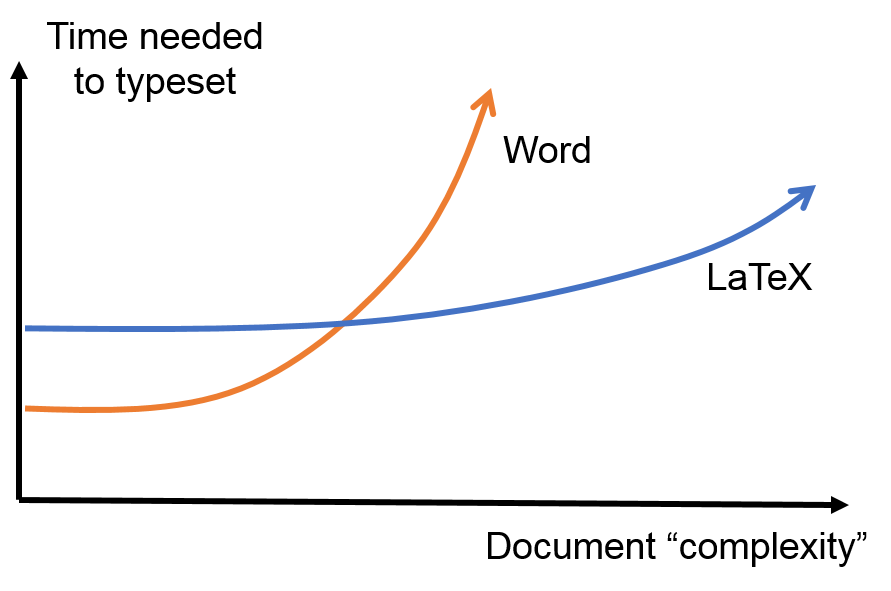
\includegraphics[width=0.75\textwidth]{word_vs_latex.png}
    \caption{Word v.s. Latex}
    \label{label}
  \end{center}
\end{figure}

\end{document}
